\subsection{Fuzzy halmazok alapjai, műveletek fuzzy halmazokon.}

Fuzzy: homályos, életlen

\textbf{Fuzzy halmaz:}
\begin{itemize}
    \item elmosódott határ (pl. magas emberek, ki mennyire számít magasnak?)
    \item részleges tagság: 0 és 1 között mennyire tartozik bele
    \item tagsági függvény ($\mu$): mennyire tartozik x halmazba?
    \item \textbf{nyelvi változó}: olyan változó, melynek értékei szavak, vagy mondatok valamilyen természetes, vagy mesterséges nyelven
    \item pl. az életkor, ha a felvett értékek nem numerikusak: nagyon fiatal, középkorú, idős, \dots
    \item karakterisztikus függvény: vagy benne van a halmazban, vagy nem
    \item példa: emberek magassága -- 3 fuzzy halmaz, van átfedés köztük
\end{itemize}

\begin{center}
    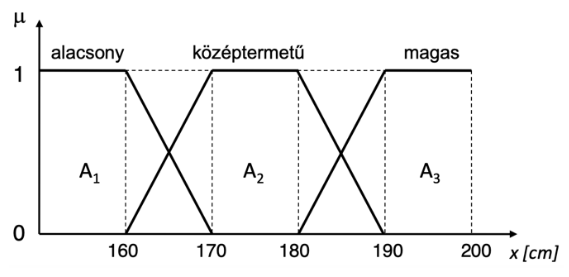
\includegraphics[width=0.8\textwidth]{res/imgs/info_16_example.png}
\end{center}

\begin{itemize}
    \item a fuzzy halmazokból ($A_i$) készített partíció $A = \{A_i\}$ fedi az alaphalmazt, ha az alaphalmaz minden eleme legalább 1 tagsági függvényben $> 0$ tagsági értékkel szerepel
    \begin{itemize}
        \item $A_1$: alacsony
        \item $A_2$: középtermetű
        \item $A_3$: magas
    \end{itemize}
\end{itemize}

\begin{minipage}{0.5\textwidth}
\begin{itemize}
    \item az ugyanazon alaphalmazon értelmezett fuzzy partíció ($A^*$) specifikusabb a másiknál (A), ha $A^*$ minden eleme specifikusabb A elemeinél
    \item ekkor $A^*$ elemeinek száma nagyobb, mint A elemeinek száma
\end{itemize}
\end{minipage}
\begin{minipage}{0.45\textwidth}
\begin{center}
    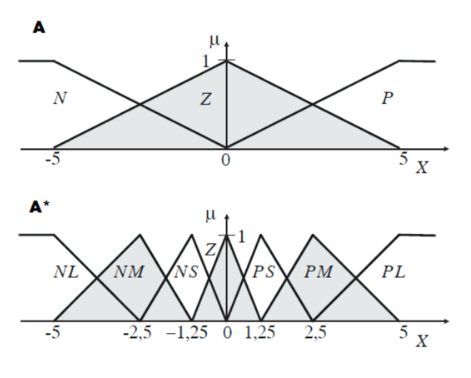
\includegraphics[width=0.9\textwidth]{res/imgs/info_16_partitions.png}
\end{center}
\end{minipage}

\begin{itemize}
    \item fuzzy halmaz -- \textbf{definíciók}:
    \begin{itemize}
        \item \textbf{mag}: $core(A) = \{x \in X \mid \mu_A(x) = 1\}$
        \item \textbf{tartó}: $supp(A) = \{x \in X \mid \mu_A(x) > 0\}$
        \item $\alpha$\textbf{-vágat}: $A_\alpha = \{x \in X \mid \mu_A(x) \ge \alpha\}$
        \item \textbf{szigorú }$\alpha$\textbf{-vágat}: $A_{\alpha+} = \{x \in X \mid \mu_A(x) > \alpha\}$
        \item \textbf{magasság}: $h(A) = \sup_{x \in X} \mu_A(x)$
        \item \textbf{$\alpha=0$-nál a tartót, $\alpha=1$-nél a magot kapjuk}
    \end{itemize}
\end{itemize}

\textbf{Példa:}
\begin{center}
    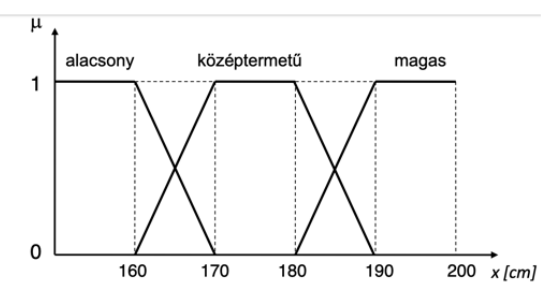
\includegraphics[width=0.8\textwidth]{res/imgs/info_16_example_calcs.png}
\end{center}
\begin{itemize}
    \item $\text{mag}(\text{középtermetű}) = [170; 180]$
    \item $\text{tartó}(\text{középtermetű}) = (160; 190)$
    \item $\text{középtermetű}_\alpha = [160+10\alpha; 190-10\alpha]$
    \item $\text{középtermetű}_{\alpha+} = (160+10\alpha; 190-10\alpha)$
    \item $\text{magasság}(\text{középtermetű}) = 1$
\end{itemize}

\textbf{Műveletek fuzzy halmazokon:}

\begin{minipage}{0.5\textwidth}
\begin{itemize}
    \item \textbf{Unió} (\textcolor{red}{s-norma}): \\
    $\mu_{A \cup B}(x) = \max(\mu_A(x), \mu_B(x))$
    \item \textbf{Metszet} (\textcolor{red}{t-norma}): \\
    $\mu_{A \cap B}(x) = \min(\mu_A(x), \mu_B(x))$
    \item \textbf{Komplemens} (\textcolor{red}{c}): \\
    $\mu_{\overline{A}}(x) = 1 - \mu_A(x)$
\end{itemize}
\end{minipage}
\begin{minipage}{0.45\textwidth}
\begin{center}
    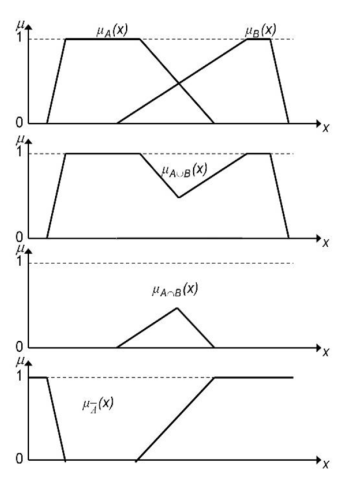
\includegraphics[width=\textwidth]{res/imgs/info_16_operations.png}
\end{center}
\end{minipage}

\textbf{c, t és s validálása:}
\begin{itemize}
    \item a komplemenst (c), t és s normákat definiáló képletek akkor alkotnak duális hármast, ha a de morgan azonosságok igazak:
    \begin{align*}
        c(t(a, b)) &= s(c(a), c(b)) \\
        c(s(a, b)) &= t(c(a), c(b))
    \end{align*}
\end{itemize}